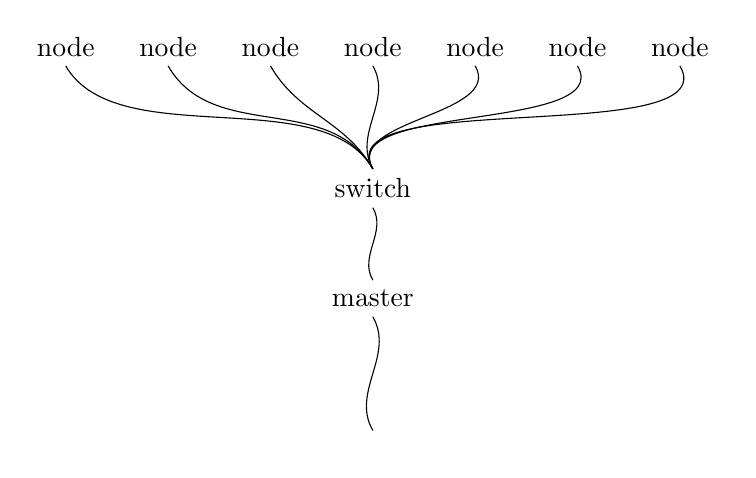
\begin{tikzpicture}[node distance=8mm,
node/.append style={xshift=5mm},
master/.append style={yshift=-.6cm},
switch/.append style={yshift=-1cm},
internet/.append style={yshift = -1cm}
]

\tikzstyle{sample} = [-,thin]

  \node (node0)   [node]                {node};
  \node (node1)   [node,right of=node0 ]                {node};
  \node (node2)   [node,right of=node1 ]                {node};
  \node (node3)   [node,right of=node2 ]                {node};
  \node (node4)   [node,right of=node3 ]                {node};
  \node (node5)   [node,right of=node4 ]                {node};
  \node (node6)   [node,right of=node5 ]                {node};
  \node (switch)   [switch,below of=node3]                {switch};
  \node (master)   [master,below of=switch]                {master};
  \node (internet)   [internet,below of=master]                {};

\path[sample] (node0.south) edge[out=-60,in=120,looseness = 0.8] (switch.north);
\path[sample] (node1.south) edge[out=-60,in=120] (switch.north);
\path[sample] (node2.south) edge[out=-60,in=120] (switch.north);
\path[sample] (node3.south) edge[out=-60,in=120] (switch.north);
\path[sample] (node4.south) edge[out=-60,in=120] (switch.north);
\path[sample] (node5.south) edge[out=-60,in=120,looseness = 0.85] (switch.north);
\path[sample] (node6.south) edge[out=-60,in=120,looseness = 0.75] (switch.north);

\path[sample] (switch.south) edge[out=-60,in=120] (master.north);

\path[sample] (master.south) edge[out=-60,in=120] (internet.north);

\end{tikzpicture}
